\chapter{Introduction}

\minitoc

\section{Background}

% TODO: 

The ability to precisely introduce mutations of various types and lengths into specified locations of the genome has profound influence in medical science and the broader field of biology, and has been a long-standing goal of many researchers. It can help to elucidate the function of genes and their regulatory elements, provide clinical interpretation of human gene variants and to develop new treatments for diseases including genetic disorders and cancer\cite{petraityteGenomeEditingMedicine2021,dasCRISPRBasedTherapeutics2022,portoBaseEditingAdvances2020}. 

The discovery of the CRISPR (clustered regularly interspaced short palindromic repeats) and CRISPR-associated protein (Cas) system in the early 2000s was a major step towards this goal. The CRISPR system is an RNA-guided adaptive immune systems in bacteria and archaea providing acquired immunity against foreign nucleic acids\cite{jiangCRISPRCas9Structures2017}. The CRISPR-Cas system works in two steps. In the adaptation step, the system acquires a short sequence of the foreign DNA(protospacer) and derive new complimentary spacers from it. Then, in the interference step, the system uses the acquired spacers to recognize and cleave the foreign DNA with the help of Cas proteins\cite{garneauCRISPRCasBacterial2010}. 

Due to its ability to recognize and introduce scissions in specific locations of the genome, the CRISPR system and a particular Cas protein, Cas9, have been harnessed as a powerful tool for genome editing. CRISPR-Cas9 uses a similar two-step process to introduce mutations in the genome, with its components shown in Figure \ref{fig:crispr-hdr}. In the first step, the Cas9 protein is guided to the target site by a typically 20bp long single guide RNA (sgRNA) that is complementary to the target site(protospacer) adjacent to the protospacer adjacent motif (PAM) required by Cas9. In the second step, the Cas9 protein introduces a double-strand break (DSB) in the target site, which is then repaired by the cell's endogenous repair machinery. For the desired edit to be installed, a single-strand or double strand DNA(ssDNA/dsDNA) donor can be provided in the second step\cite{richardsonEnhancingHomologydirectedGenome2016,jasinRepairStrandBreaks2013}. The endogenous homology directed repair (HDR) system can then use the donor DNA as template and install the intended edits\cite{hsuDevelopmentApplicationsCRISPRCas92014}. However, a competing repair pathway, the non-homologous end joining (NHEJ) pathway, is more prevalent in mammalian cells and often introduces unintended insertions or deletions (indels) at the target site\cite{changNonhomologousDNAEnd2017}. Although various improvements to the Cas9 proteins and gRNA have been made over the years, the CRISPR-Cas9 is still mostly used to introduce disruptions into the genome rather than installing precise edits due to its high indel rate\cite{kantorCRISPRCas9DNABaseEditing2020,koeppelPredictionPrimeEditing2023}.

% subfigure side by side
\begin{figure}[ht]
    \centering
    \subfigure[CRISPR-Cas9 HDR]{
        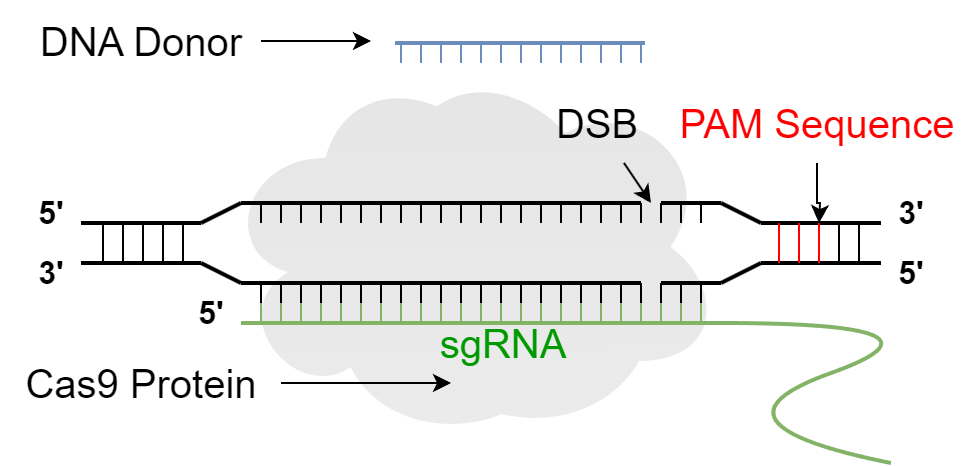
\includegraphics[width=0.46\textwidth]{dissertation-crispr-hdr.png}
        \label{fig:crispr-hdr}
    }
    \subfigure[Base Editor]{
        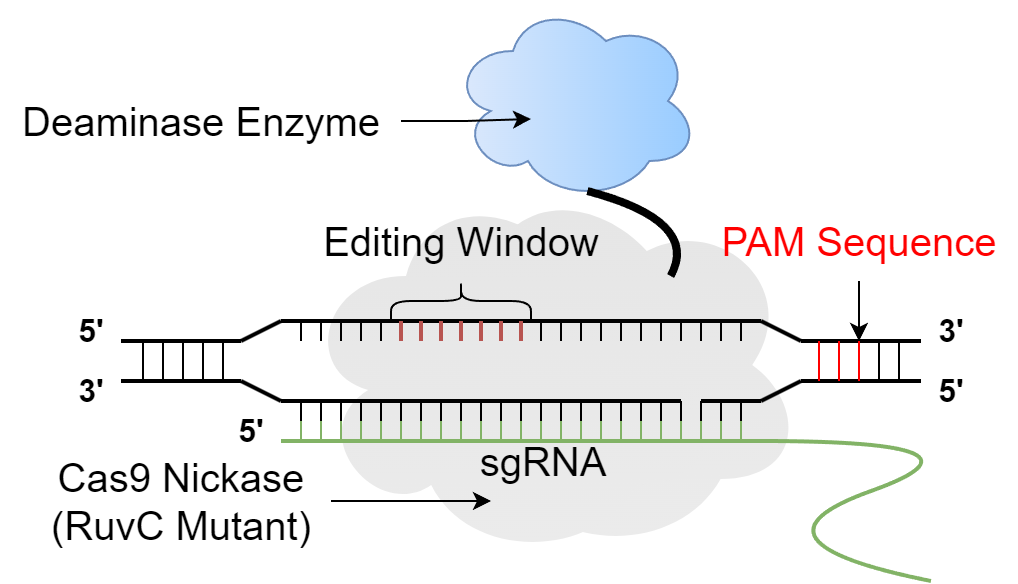
\includegraphics[width=0.46\textwidth]{dissertation-base-editor.png}
        \label{fig:base-editor}
    }
    \caption{Components for \textbf{(a)} CRISPR-Cas9 HDR  and \textbf{(b)} Base Editor  systems.}
    \label{fig:crispr-base-editor}
\end{figure}

To avoid the inefficiencies produced by DSB while still leveraging the targeting capabilities of CRISPR system, the nickase versions of Cas9 proteins were developed. Cas9 nickase is a mutated version of the Cas9 protein that only cleaves the binding(RuvC mutation) or opposite(HNH mutation) strand of the guide RNA\cite{dasCRISPRBasedTherapeutics2022}. David Liu and his team developed the base editing system that uses the RuvC mutated Cas9 nickase to introduce point mutations in the genome, shown in Figure \ref{fig:base-editor}\cite{gaudelliProgrammableBaseEditing2017}. The base editing system consists of a fusion protein of the Cas9 nickase and a deaminase enzyme, and a sgRNA that guides the fusion protein to the target site. The deaminase enzyme converts a specific nucleotide within the editing window to another, and the Cas9 nickase introduces a nick in the non-edited strand to encourage the cell's endogenous repair machinery to use the edited strand as a template and permanently install the edit into the genome.

The base editors have been improved to be able to introduce point mutation within the editing window with relatively high efficiency\cite{portoBaseEditingAdvances2020}. However, they are only designed to introduce single-nucleotide variants into DNA or RNA, and are not capable of inserting and deleting sequences. To address this limitation and acquire a truly versatile genome editing tool, Liu's lab further developed prime editors\cite{liudavidr.SearchandreplaceGenomeEditing2019}. Prime editors are capable of introducing all 12 possible types of point mutations, as well as insertion and deletion of sequences up to a couple thousand base pairs in length\cite{linHighefficiencyPrimeEditing2021}. 

Prime editors consist of a fusion protein of SpCas9 (Streptococcus pyogenes) nickase and a MMLV reverse transcriptase, as well as a prime editing guide RNA (pegRNA), illustrated in Figure \ref{fig:prime-editor}. The SpCas9  nickase is a popular variant of Cas9 protein in recent years, mostly due to its high targetability (recognizing the common NGG PAM sequence, where N can be any nucleotide) and low off-target effects\cite{waltonUnconstrainedGenomeTargeting2020}. Similar to the sgRNA used by base editors, the pegRNA contains a nicking single guide RNA (ngRNA) at the $5'$ end. On the $3'$ end, however, pegRNA has a unique RNA sequence that encodes the desired edit. The $3'$ sequence can be divided into two parts: the primer binding site (PBS) and the reverse transcription template (RTT) consists of the intended edit surrounded by the left/right homology arms (LHA/RHA, RHA also called RTT overhang). As their names suggest, the PBS and RTT are used to prime the reverse transcription process, while the LHA and RHA are unedited sequences used to facilitate the integration of the edited sequence into the genome. The two ends of the pegRNA are connected by a crRNA scaffold sequence, which should have no participation in the prime editing process. 

\section{Process of Prime Editing}

\label{sec:prime-editing-process}

\begin{figure}[ht]
    \centering
    \subfigure[]{
        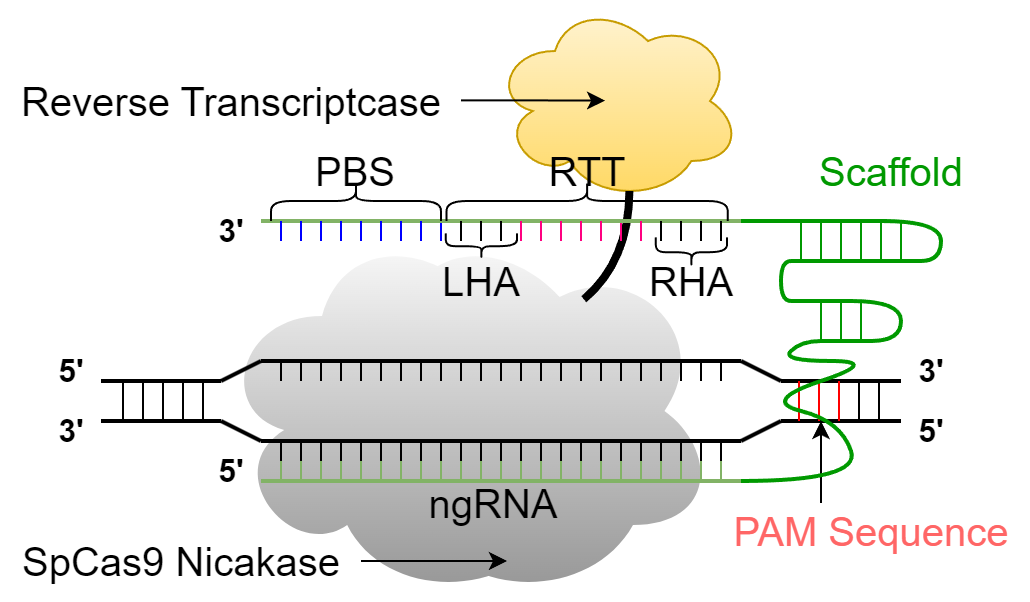
\includegraphics[width=0.46\textwidth]{dissertation-prime-editing-process-1.png}
        \label{fig:prime-editor}
    }
    \subfigure[]{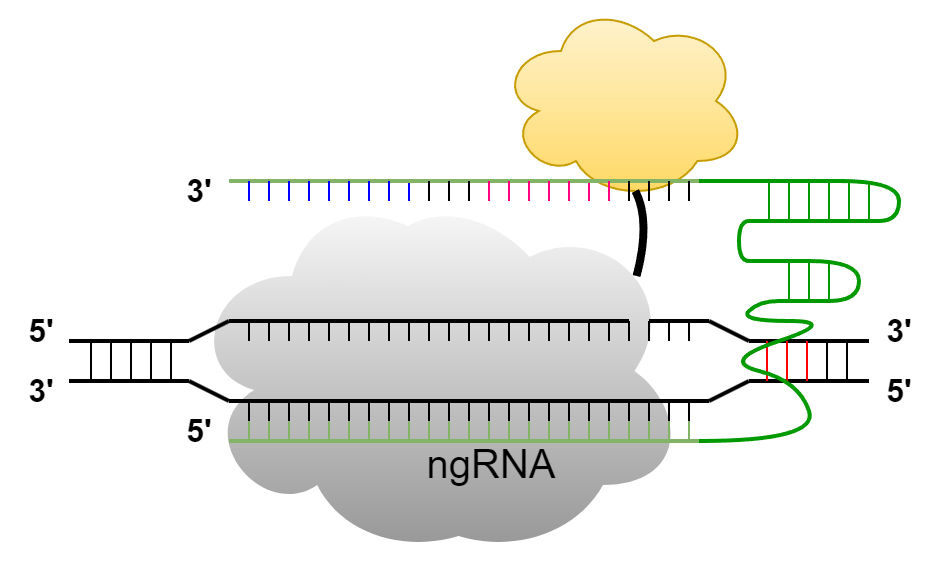
\includegraphics[width=0.46\textwidth]{dissertation-prime-editing-process-2.png}}
    \subfigure[]{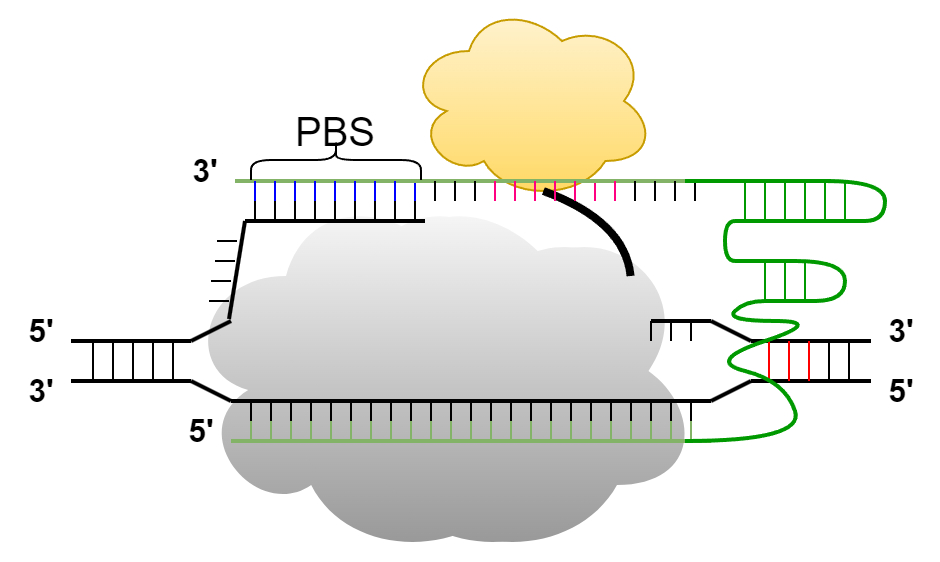
\includegraphics[width=0.46\textwidth]{dissertation-prime-editing-process-3.png}}
    \subfigure[]{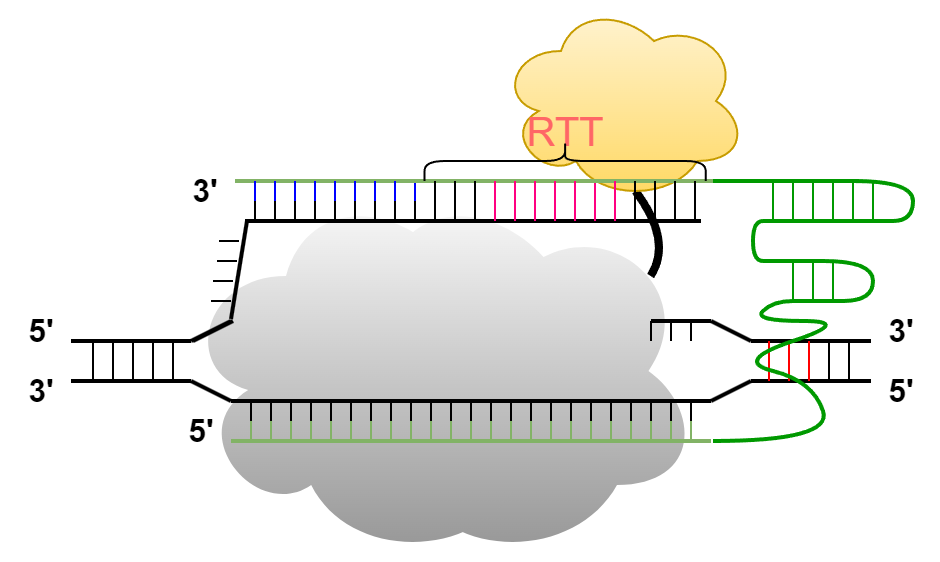
\includegraphics[width=0.46\textwidth]{dissertation-prime-editing-process-4.png}}
    \subfigure[]{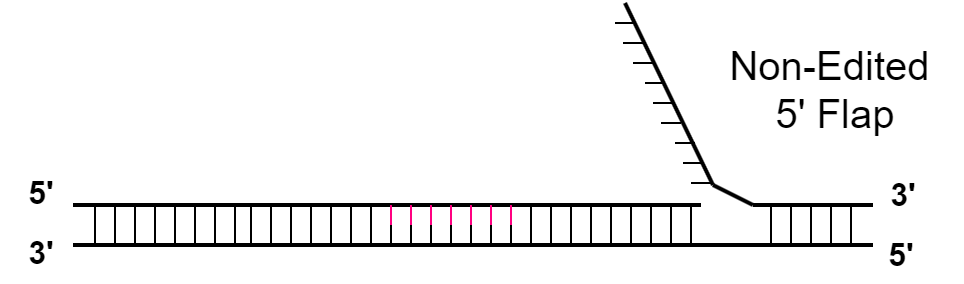
\includegraphics[width=0.46\textwidth]{dissertation-prime-editing-process-5.png}}
    \subfigure[]{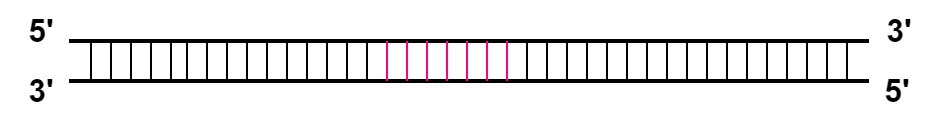
\includegraphics[width=0.46\textwidth]{dissertation-prime-editing-process-6.png}}
    \caption[Components of Prime Editor \textit{(a)} and the process of prime editing \textit{(a-f)}]{Components of Prime Editor \textit{(a)} and the process of prime editing \textit{(a-f)}: \textbf{(a)} ngRNA binds to the target DNA loci; \textbf{(b)} SpCas9 introduces nick 3-4 bp upstream of PAM; \textbf{(c)} The now exposed strand hybridizes with the PBS sequence in the pegRNA; \textbf{(d)} The RTT in the pegRNA is reverse transcribed into the target DNA; \textbf{(e)} The edited strand anneals to the non-edited strand; \textbf{(f)} The endogenous repair machinery incorporates the edited strand into the genome.}
    \label{fig:prime-editing-process}
\end{figure}

Numerous prime editors has been developed since the first generation(PE2, PE3) was introduced in 2019, including PE4 and PE5 with additional MLH1dn protein to inhibit the adverse mismatch repair pathway, as well as PE2-max and PE4-max with updated SpCas9 and reverse transcriptase\cite{liuPrimeEditingPrecise2023}. Despite their differences, all of the prime editors follow a similar multi-stage process illustrated in \autoref{fig:prime-editing-process}. 

The prime editing process starts with the denaturing (separation of the two strands) of target DNA loci. This allows ngRNA to bind to the complementary sequence immediately upstream of the protospacer adjacent motifs (PAM) required for successful annealing (binding of two complementary strands of DNA or RNA). The Cas9 nickase can then nick the exposed strand of the target DNA, creating a floating 3' end that can be used as a primer for the reverse transcription process. The PBS sequence in the pegRNA binds to the exposed 3' end, priming the reverse transcription of the RTT. 

Both the reverse transcribed 3' flap and non-edited 5' flat could anneal to the protospacer, and would result in a equilibrium of 3' and 5' flaps. If the edited 3' flap was excised, target would not be edited and can be processed again with prolonged editing. If the 5' flap was correctly excised, then we move on to the final step where the endogenous cellular repair system permanently incorporates the edited strand into the genome by repairing the mismatched base pairs. To stimulate the replacement of the non-edited strand, PE3 and PE5 have an additional sgRNA that guides the PE2 enzyme to nick the non-edited strand.

The reverse transcription mechanism gives prime editors an additional advantage. It can change bases far (at least 33bp) from the site of nick, instead of the narrow editing window of base editors. This allows prime editors to have lower constraint on the relative location of the PAM sequence, further increasing the versatility\cite{liuPrimeEditingPrecise2023}.

\section{In-silico Prediction of Prime Editing Outcome}

\label{sec:motivation}

More than 6,000 disorders are known to be caused by various types of mutations in the genome, with around 300 new genetic disorders being discovered each year\cite{petraityteGenomeEditingMedicine2021}. Due to its versatility, prime editing has the potential to correct up to 90\% of these disorder-inducing mutations\cite{kantorCRISPRCas9DNABaseEditing2020}, and the coverage is still increasing with new SpCas9 variants that have less and less PAM sequence constraints\cite{waltonUnconstrainedGenomeTargeting2020}. However, for prime editors to be useful in treating human diseases in clinical setting, it is crucial to have the highest possible accuracy with minimal off-target effects during the edits. 

The efficiency of prime editing can vary greatly across different target sites and pegRNA designs\cite{liudavidr.SearchandreplaceGenomeEditing2019}. Empirical approaches have been used to find the prime editor given a target edit, which involves testing a large number of combinations of ngRNA, PBS and RTT sequences repeatedly to find the optimal combination that yields the highest editing efficiency.

This is a laborious and time consuming process even for simpler editing tools such as base editors. With the more complicated process of prime editing, the search space is even larger. The lack of efficient optimization process can significantly limit the practicality in the clinical setting, especially in territories with an existing shortage of medical workers. As a result, in-silico optimization methods are highly desirable and has garnered the interest of many researchers.

Previous in-silico methods can be divided into two catagories: hypothesis driven models that use hard-coded rules to calculate the efficiency of a given edit\cite{hsuPrimeDesignSoftwareRapid2021,hwangPEDesignerPEAnalyzerWebbased2021}, and learning-based models that use machine learning to predict the editing outcome. 
The learning-based methods can be further divided into another two groups: the conventional machine learning methods that use hand-crafted features extracted from the sequence and prime editors\cite{liEasyPrimeMachineLearning2021,koeppelPredictionPrimeEditing2023}, as well as the deep learning methods that use the raw sequence data as part of their input\cite{yuPredictionEfficienciesDiverse2023,kimPredictingEfficiencyPrime2021, mathisPredictingPrimeEditing2023}. 

Each category has their own strengths and weaknesses in performance and efficiency. Hypothesis driven and conventional machine learning algorithms are more efficient to train due to the much smaller input size and the lower complexity of the computation. However, hypothesis based methods struggle to unbiasedly optimize the weights attributed to each feature\cite{liEasyPrimeMachineLearning2021}, while conventional machine learning algorithms loses the DNA context data that can be informative to prime editor optimization. 

The deep learning methods require a much larger dataset to train and are computationally more expensive to train and use. They also need more expertise to design and tune, and are more prone to overfitting due to the large number of parameters. However, their superior performance in the prime editing efficiency prediction task has been convincingly demonstrated by a number of models in recent years.

% TODO: overview of DeepPE, DeepPrime, PRIDICT 1 and 2

\subsection{DeepPE and DeepPrime convolutional neural network}

\begin{figure}
    \centering
    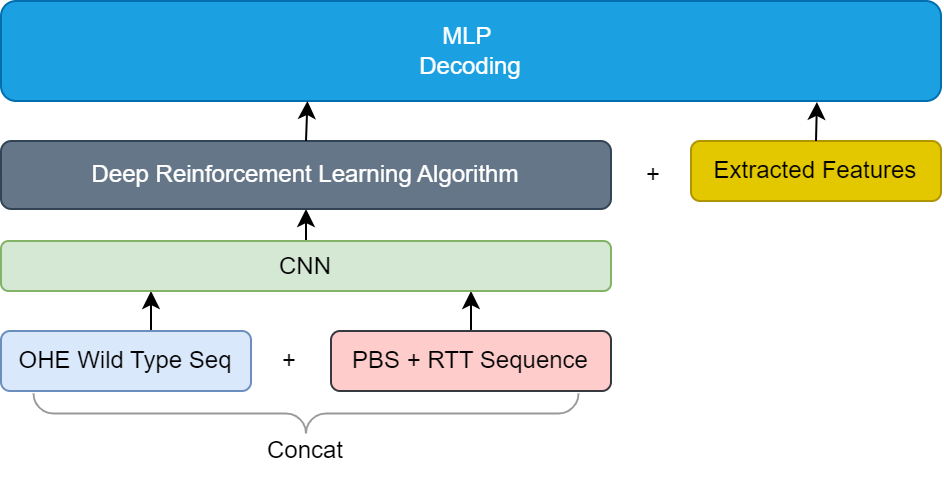
\includegraphics[width=0.7\textwidth]{DeepPE-simplified.png}
    \caption[DeepPE architecture]{DeepPE architecture. The input to the CNN is the one-hot encoded wild type and mutated DNA sequences concatenated with the extension RNA sequence. The output of the CNN is concatenated with the extracted features from the pegRNA sequence and the target site, and fed into the final MLP to predict the editing efficiency. Note that a deep reinforcement learning model was used here instead of a pooling layer to maintain local context information.}
    \label{fig:deeppe}
\end{figure}

DeepPE (\autoref{fig:deeppe}) was one of the earliest attempts at leveraging deep learning to achieve above par performance in predicting prime editing outcomes\cite{kimPredictingEfficiencyPrime2021}. It is a convolutional neural network that takes the stacked one-hot encoded wild type and  mutated DNA sequences, the extension RNA sequence as well as a number of features extracted from pegRNA sequence and the target site as input. Despite its simple architecture, DeepPE managed to outperform the conventional machine learning models in terms of Pearson's r and Spearman's R. This indicated that the deep learning model was able to better capture the complex interactions between the sequence data and the editing efficiency compared to using the extracted features alone. It was however very limited in terms of the types of edits it can predict, with the base model only capable of predicting the efficiency of G to C replacement at 5bp upstream of the nick. Additional models were trained to predict other types of edits, and most of them also only support one single specific edit.

\begin{figure}
    \centering
    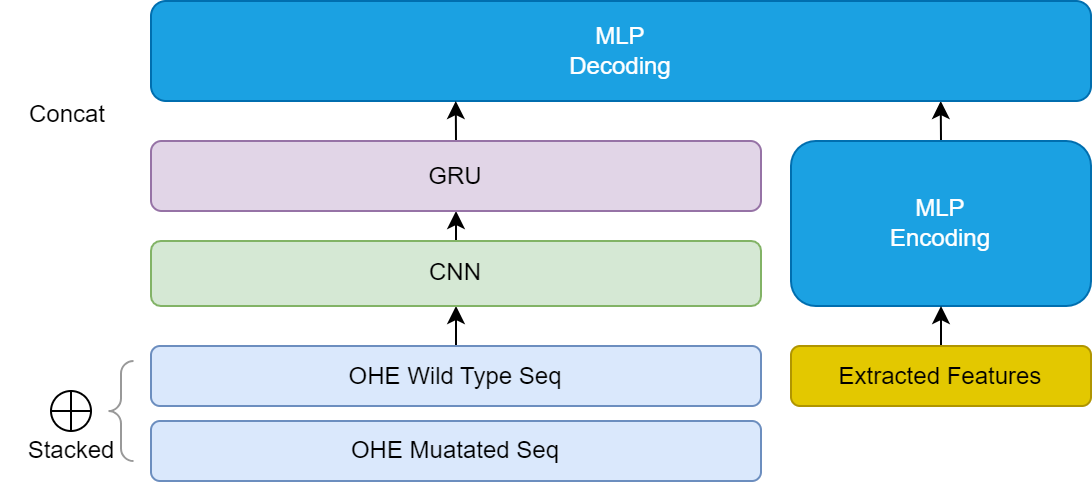
\includegraphics[width=0.85\textwidth]{DeepPrime-simplified.png}
    \caption[DeepPrime architecture]{DeepPrime architecture, updated from DeepPE. The CNN now uses a more conventional pooling layer, followed by a RNN GRU (Gated Recurrent Unit). The convolutional and recurrent layers take the stacked one-hot encoded wild type and mutated DNA sequences as input, and the output is concatenated with the extracted features processed by a MLP module. The concatenated output is then fed into another MLP to predict the editing efficiency.}
    \label{fig:deepprime}
\end{figure}

DeepPrime is a further attempt made by the same group to improve the performance and capabilities of DeepPE, leveraging the much bigger dataset as well as an improved architecture design\cite{yuPredictionEfficienciesDiverse2023}.
Noticing that stacking the additional PBS-RTT sequence did not improve the performance of DeepPE and added further constraint on pegRNA design (CNN only accept fixed length input), DeepPrime only used the wild type and mutated sequences as input to the deep learning model, and added a separate MLP (Multi Layer Perceptron) to process the computed features instead of directly concatenated the features onto the CNN output as DeepPE did. The output of the MLP was then concatenated with the output of the CNN (Convolutional Neural Network) that processed the sequence data, and fed into the final MLP to predict the editing efficiency. 

DeepPrime achieved far superior performance to DeepPE, while at the same time, one single model can now predict all types of edits for a cell line and prime editor pair existing in the dataset. This enabled the training process to take advantage of the shared features between different edits (further enhancing performance) and significantly improve the ease of use.

\subsection{PRIDICT 1 and 2 bidirectional GRU}

At around the same time DeepPrime was published, the PRIDICT model was developed by Mathis et al from the Schwank lab at the University of Zurch, and used RNN (Recurrent Neural Network) instead of CNN to process the sequence data\cite{mathisPredictingPrimeEditing2023}. The model uses a bidirectional GRU (Gated Recurrent Unit) to process the sequence data, whose output is pooled by a pair of global (whole sequence) and local (RTT region) attention(\autoref{fig:pridict}). Similar to DeepPrime, the features are encoded using a MLP and the output of the two models are then concatenated and fed into the final MLP to predict the editing efficiency.

\begin{figure}
    \centering
    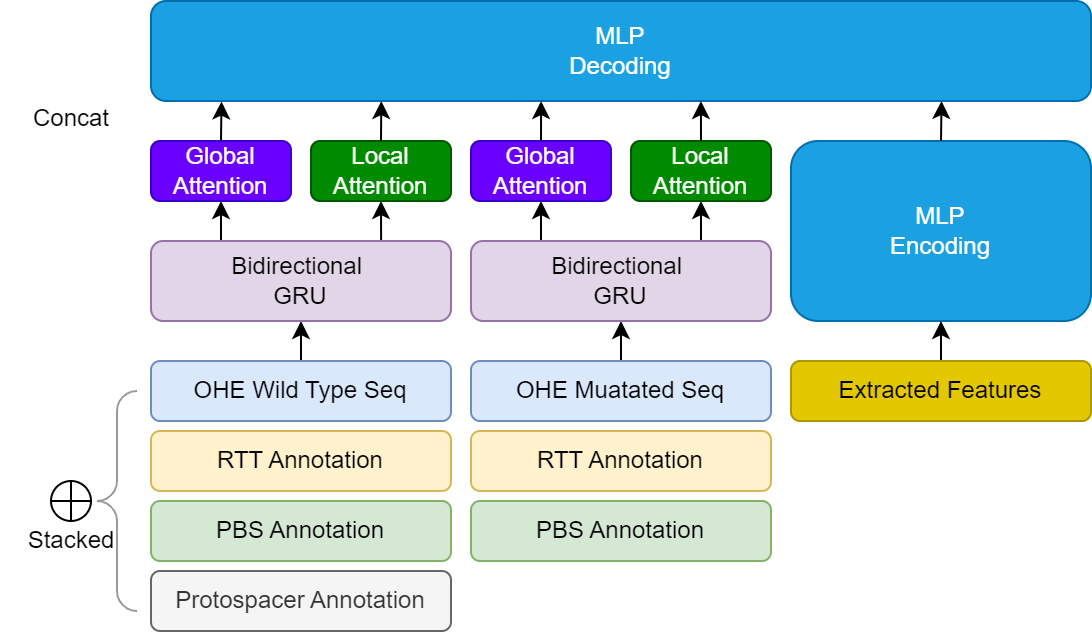
\includegraphics[width=0.85\textwidth]{pridict-simplified.png}
    \caption[PRIDICT architecture]{PRIDICT architecture. The input to the RNN is the one-hot encoded wild type and mutated DNA sequences, stacked with RTT, PBS, Protospacer(only for wild type) annotations. The annotation sequences are boolean sequences that indicate the functionality of each nucleotide in the sequence. The output of the RNN is processed by two attention heads, a global one that process the entire sequence and a local one that masks out all regions other than RTT. }
    \label{fig:pridict}
\end{figure}

Leveraging the 

This RNN based model was able to achieve similar performance to DeepPrime on their dataset. Additionally, thanks to the far more diverse edits in the dataset with much longer inserts and deletes, PRIDICT was more capable in the laboratory setting where insertion and deletions are reaching hundreds of base pairs in length\cite{liuPrimeEditingPrecise2023}.

\section{Study Objective}

(Rewrite)

The development of these models inspired me to further explore the potential of deep learning models in predicting prime editing outcomes. In this study, I aim to develop a deep learning model that is on par or even better than the existing models in predicting prime editing outcomes for a wide range of cell lines and edit types. 

I will also explore the possibility of using ensemble learning to improve the performance of the models, and investigate the potential of using the model to predict the efficiency of prime editing outcomes for cell lines and edit types that are not present in the training dataset. 

The best performing trained model would be presented as a web application that can be used by researchers to predict the efficiency of prime editing outcomes for their own cell lines and edit types.